\documentclass[12pt]{article}%
\usepackage{amsfonts}
\usepackage{fancyhdr}
\usepackage{comment}
\usepackage[a4paper, top=2.5cm, bottom=2.5cm, left=2.2cm, right=2.2cm]%
{geometry}
\usepackage{times}
\usepackage{amsmath}
\usepackage{changepage}
\usepackage{stfloats}
\usepackage{amssymb}
\usepackage{graphicx}
\usepackage{indentfirst}

\setlength{\parindent}{2em}
\setcounter{MaxMatrixCols}{30}
\newtheorem{theorem}{Theorem}
\newtheorem{acknowledgement}[theorem]{Acknowledgement}
\newtheorem{algorithm}[theorem]{Algorithm}
\newtheorem{axiom}{Axiom}
\newtheorem{case}[theorem]{Case}
\newtheorem{claim}[theorem]{Claim}
\newtheorem{conclusion}[theorem]{Conclusion}
\newtheorem{condition}[theorem]{Condition}
\newtheorem{conjecture}[theorem]{Conjecture}
\newtheorem{corollary}[theorem]{Corollary}
\newtheorem{criterion}[theorem]{Criterion}
\newtheorem{definition}[theorem]{Definition}
\newtheorem{example}[theorem]{Example}
\newtheorem{exercise}[theorem]{Exercise}
\newtheorem{lemma}[theorem]{Lemma}
\newtheorem{notation}[theorem]{Notation}
\newtheorem{problem}[theorem]{Problem}
\newtheorem{proposition}[theorem]{Proposition}
\newtheorem{remark}[theorem]{Remark}
\newtheorem{solution}[theorem]{Solution}
\newtheorem{summary}[theorem]{Summary}
\newenvironment{proof}[1][Proof]{\textbf{#1.} }{\ \rule{0.5em}{0.5em}}

\usepackage{mathtools}

\newcommand{\Q}{\mathbb{Q}}
\newcommand{\R}{\mathbb{R}}
\newcommand{\C}{\mathbb{C}}
\newcommand{\Z}{\mathbb{Z}}

\begin{document}

\title{MATH2040C Homework 7}
\author{ZHENG Weijia (William, 1155124322)}
\date{April 25, 2021}
\maketitle

\large

\section{Section 6.3, Q3(c)}

\begin{figure}[htp]
    \centering % 图片居中
    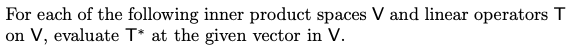
\includegraphics[width = 16cm]{img/Q1a.png}
    \includegraphics*[width = 15cm]{img/Q1b.png}
    %\caption{Section 6.1 Q8}
    %\label{fig:figure1label}
\end{figure}


The first thing we need to do is to find a orthonormal basis for $V$.

A basis for $V$ is $\alpha=\{1,t\}.$ Note that $\int_{-1}^{1}1\cdot t ~dt =0.$
Therefore $\alpha$ is an orthogonal basis. Applying the Gram-Schmidt process, we can 
generate an orthonormal basis $\beta=\{\frac{1}{\sqrt{2}},\frac{\sqrt{3}t}{\sqrt{2}} \}$.

Then according to Remark 16.3, we can have 
$$T^* (g(t))=\sum_{i=1}^n \overline{\langle T(v_i),g(t) \rangle} v_i.$$

With $T(\frac{1}{\sqrt{2}})=\frac{3}{\sqrt{2}}$. 
And $T(\sqrt{\frac{3}{2}}t)=\sqrt{\frac{3}{2}}+3\sqrt{\frac{3}{2}}t.$. 

Therefore, $$T^*(g(t))=\frac{3}{2}\int_{-1}^1 g(t)dt + \frac{3}{2}t\int_{-1}^1 (1+3t)g(t)dt.$$

The given vector is $f(t)=4-2t.$ Hence the answer should be 
$$T^*(4-2t)=12+6t.$$

Done.



\newpage

\section{Section 6.3, Q13}

\begin{figure}[htp]
    \centering % 图片居中
    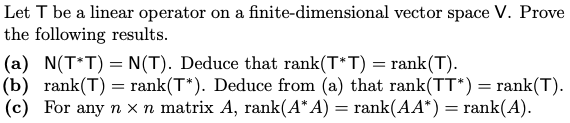
\includegraphics[width = 16cm]{img/Q2.png}
    %\caption{Section 6.1 Q8}
    %\label{fig:figure1label}
\end{figure}

\subsection{(a)}
Note that $\forall x \in N(T),$ $$T^*Tx = T^*(Tx)=T^*(0)=0.$$

Therefore $x\in N(T^*T).$ Hence $N(T) \subset N(T^*T).$

Forall $y \in N(T^*T), $ consider the norm of $Ty:$ 
$$||Ty||^2=\langle Ty,Ty \rangle=\langle y, T^*Ty \rangle = \langle y,0 \rangle=0.$$

Which implies that $Ty=0.$ Therefore $y \in N(T).$ Hence $N(T^*T) \subset N(T).$

Based on all above, $N(T^*T)=N(T).$

Recall that $T \in \mathcal{L}(V).$ Hence $T:V \to V.$ And according to $\forall y \in V,$
$$T^*(y)=\sum_{i=1}^n \overline{\langle T(v_i),y \rangle} v_i.$$

We know that $T^*:V \to V.$ Therefore $T^*T:V \to V.$

Applying the rank nullity theorem, we have that 
$$\dim{V} = rank(T^*T)+\dim{N(T^*T)}~,~\dim{V} = rank(T)+\dim{N(T)}.$$

Using the just proved fact $N(T^*T)=N(T),$ we can simply deduce $$rank(T^*T)=rank(T).$$

\subsection{(b)}
By changing name of the identity in (a), we can have $N(TT^*)=N(T^*)$ and $rank(TT^*)=rank(T^*).$

Notice that $$rank(T)=rank[T]_\beta=rank[T]_\beta^*=rank[T^*]_\beta=rank(T^*).$$

And then $rank(TT^*)=rank(T)$ follows.

\subsection{(c)}
From (b), $rank(AA^*)=rank(A)$ follows naturally. 

And note that $(AA^*)^* =A^*A$, then $$rank(AA^*)=rank(A^*A).$$

Therefore, $$rank(AA^*)=rank(A^*A)=rank(A).$$

Done.




\newpage

\section{Section 6.3, Q14}
\begin{figure}[htp]
    \centering % 图片居中
    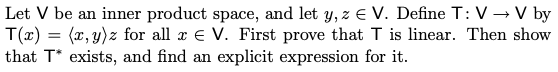
\includegraphics[width = 16cm]{img/Q3.png}
    %\caption{Section 6.1 Q8}
    %\label{fig:figure1label}
\end{figure}





\end{document}